\subsection{问题二求解思路}

场景 B 有核间同步机制，同一核心上的全部子图合并成一个 Task（图~\ref{fig:sceneAB}(b)）。与场景 A 相比有三处变化。同核子图之间的数据留在 L1/UB 中直接复用，不再经 DDR 往返，同核边界不产生任何搬运。跨核依赖由源核插入 COPY\_OUT、目标核插入 COPY\_IN，目标 COPY\_IN 要在源 COPY\_OUT 完成后再等 $\delta_B=500$ 周期才进入就绪判定，按子图计的激活等待不再存在。全核只有一个 Task，核内调度器面对的是该核全部子图拼成的大图，跨越多个子图的驻留数据会一直占着缓存，容量不够时就插入换入换出。

前两处变化让细分切图变得便宜，第三处又给细分和合并都设了限。求解思路是：保留问题一的决策变量与合法性约束，把边界搬运从子图边界改为核边界，把时间约束从子图激活改为操作级的跨核同步，并加入缓存驻留约束；由修正后的模型判断参数应向哪个方向移动，再沿用问题一的三种构造算法与选优框架。后处理中成组合并的作用在场景 B 下有所不同，需要重新分析。由于问题二、三同属场景 B，两问的候选方案还可以互相复评。

\subsection{问题二模型建立}\label{sec:p2-model}

\subsubsection{边界搬运量的修正}

场景 B 下只有跨核的张量需要搬运。把式 \eqref{eq:copies-A} 中的子图映射 $\sg$ 换成核心映射 $\core$，得到
\begin{equation}
  n^{\mathrm{in}}_t=\big|\core(U_t)\setminus \core(P_t)\big|,\qquad
  n^{\mathrm{out}}_t=\big|\{\,n\in \core(P_t):\ t\in T_{\mathrm{out}}\ \text{或}\ \core(U_t)\setminus\{n\}\ne\varnothing\,\}\big| ,
  \label{eq:copies-B}
\end{equation}
\begin{equation}
  Q_B=\sum_{t\in T} s_t\big(n^{\mathrm{in}}_t+n^{\mathrm{out}}_t\big)-Q_{\mathrm{orig}} .
  \label{eq:QB}
\end{equation}
推理与式 \eqref{eq:copies-A} 相同，只是边界的单位变了：场景 B 中同一核心上的子图属于同一个 Task，张量在核内生产、在核内使用时不需要搬运；只有当某个核心要用到别的核心生产的张量时，才需要一次读入，而生产它的核心只要有别的核心使用它（或它是图输出）就要写出一次。所以把式 \eqref{eq:copies-A} 中的子图集合 $\sg(\cdot)$ 换成核心集合 $\core(\cdot)$，就得到场景 B 的搬运次数，再逐张量求和并减去原图已有的 COPY 字节，即得式 \eqref{eq:QB}。

\begin{proposition}\label{prop:qb}
对同一份方案，场景 B 的边界搬运量不超过场景 A，即 $Q_B\le Q_A$。
\end{proposition}
\begin{proof}
核心映射是子图映射的复合，$\core(v)=\core(\sg(v))$，所以对任意操作集合 $X$ 有 $|\core(X)|\le|\sg(X)|$。对读入次数，若核心 $n\in\core(U_t)\setminus\core(P_t)$，则 $n$ 上消费 $t$ 的子图都不在 $\sg(P_t)$ 中，即 $\core(U_t)\setminus\core(P_t)\subseteq \core\big(\sg(U_t)\setminus\sg(P_t)\big)$，于是场景 B 的 $n^{\mathrm{in}}_t$ 不超过场景 A。对写出次数，场景 B 中每个计入的生产核心至少对应一个满足场景 A 计入条件的生产子图，且不同核心对应的子图互不相同，故也不超过场景 A。逐张量相加即得。
\end{proof}

命题~\ref{prop:qb} 意味着切得越细，两种场景的差距越大：子图数增加时 $Q_A$ 随子图边界增长，$Q_B$ 只随核边界增长。图~\ref{fig:trafficAB} 用同一方案在两种场景下的 \V{fig_traffic_pairs} 组配对评估验证了这一点：子图数在 512 个以上时，场景 B 的额外搬运量只有场景 A 的 \V{fig_traffic_added_ratio_4}，Makespan 为场景 A 的 \V{fig_traffic_ms_ratio_4}。

\begin{figure}[H]
  \centering
  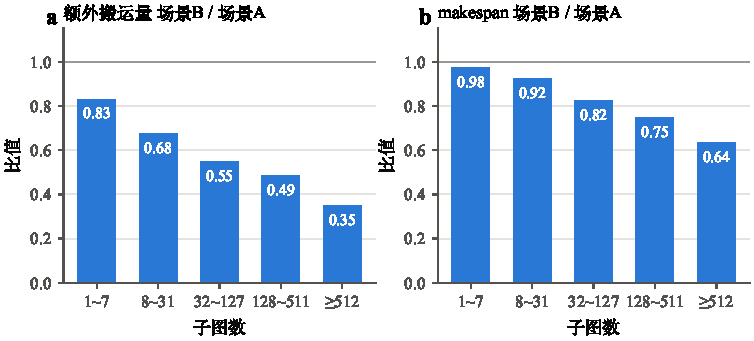
\includegraphics[width=\textwidth]{traffic_AB}
  \caption{同一方案在场景 A、B 下的配对对比（按子图数分组）}
  \label{fig:trafficAB}
\end{figure}

\subsubsection{时间模型的修正}

场景 B 中子图不再单独激活，时间约束落在操作上。对跨核依赖 $(u,v)$，设 $u$ 的输出张量为 $t$，则
\begin{equation}
  S_v\ \ge\ f_u+\frac{s_t}{B_u^{\mathrm{eff}}}+\delta_B+\frac{s_t}{B_v^{\mathrm{eff}}},
  \label{eq:sync-B}
\end{equation}
同核依赖只需 $S_v\ge f_u$。$B^{\mathrm{eff}}$ 为 COPY 执行时实际分到的带宽。式 \eqref{eq:sync-B} 按跨核数据的实际流程逐段相加：$u$ 完成后，源核的 COPY\_OUT 把 $t$ 写回 DDR，耗时 $s_t/B_u^{\mathrm{eff}}$；写完后要等同步延迟 $\delta_B$，目标核的 COPY\_IN 才进入就绪判定；再读入 $t$，耗时 $s_t/B_v^{\mathrm{eff}}$，之后 $v$ 才能开始。按题目附录 D.5，所有访问 DDR 的搬运公平共享总带宽。设时刻 $\tau$ 有 $m(\tau)$ 个 DDR 搬运在途，第 $j$ 个的剩余字节数为 $w_j(\tau)$，则每个在途搬运分到 $B/m(\tau)$ 的带宽：
\begin{equation}
  \frac{\mathrm{d}w_j}{\mathrm{d}\tau}=-\frac{B}{m(\tau)},\qquad
  e_j=\min\{\tau:\ w_j(\tau)=0\}.
  \label{eq:fair-share}
\end{equation}
从发射时刻 $a_j$ 到完成时刻 $e_j$ 对上式积分，得 $s_j=\int_{a_j}^{e_j}B/m(\tau)\,\mathrm{d}\tau$，于是这次搬运的平均带宽为
\begin{equation}
  B^{\mathrm{eff}}_j=\frac{s_j}{e_j-a_j}=\frac{1}{e_j-a_j}\int_{a_j}^{e_j}\frac{B}{m(\tau)}\,\mathrm{d}\tau\ \le\ B ,
  \label{eq:beff}
\end{equation}
不等号是因为 $m(\tau)\ge 1$。$m(\tau)$ 只在有搬运加入或完成时改变，评估程序按事件逐段结算。跨核搬运的实际耗时因此不只取决于自身字节数，还取决于同一时段有多少搬运在争用带宽，这也是式 \eqref{eq:sync-B} 中 $B^{\mathrm{eff}}$ 写不成常数的原因。沿任意一条依赖路径 $v_1\to v_2\to\cdots\to v_m$，同核的相邻操作满足 $S_{v_{i+1}}\ge f_{v_i}$，跨核的相邻操作满足式 \eqref{eq:sync-B}；由式 \eqref{eq:beff}，$B^{\mathrm{eff}}\le B$，所以每次跨核至少多出 $\delta_B+2s_t/B$。再由 $f_{v_i}\ge S_{v_i}+c_{v_i}$ 沿路径累加，若路径换核 $h$ 次，则
\begin{equation}
  M_k\ \ge\ \sum_{i=1}^{m} c_{v_i}+h\Big(\delta_B+\frac{2\,\bar s}{B}\Big),
  \label{eq:path-B}
\end{equation}
$\bar s$ 为路径上跨核张量的最小字节数。与式 \eqref{eq:path-bound} 相比，这里的代价只与换核次数有关，与子图数无关。场景 B 中真正要控制的是换核深度，同核上切出多少子图本身不付代价。

\subsubsection{缓存驻留约束}

场景 B 的另一部分代价在核内。设核心 $n$ 上合并后 Task 的操作按核内调度顺序排为 $o_1,o_2,\dots$，张量 $t$ 从生产者完成到该核上最后一个消费者开始都驻留在缓存中，驻留区间与第 $j$ 步的驻留量为
\begin{equation}
  \mathcal{L}_t=\big[f_{P_t},\ \max_{v\in U_t,\ \core(v)=n} S_v\big],\qquad
  \Phi_n(j)=\sum_{t:\ o_j\in\mathcal{L}_t} s_t .
  \label{eq:live}
\end{equation}
张量从生产出来到最后一次被该核使用之前都不能丢弃，所以它在 $\mathcal{L}_t$ 内一直占用缓存，第 $j$ 步的占用量就是所有驻留区间覆盖 $o_j$ 的张量字节之和。按张量所在的缓存分别求和，必须满足
\begin{equation}
  \Phi_n^{L1}(j)\le C_{L1},\qquad \Phi_n^{UB}(j)\le C_{UB},\qquad \forall n,\ j .
  \label{eq:resident}
\end{equation}
不满足时，调度器按“下一次使用最晚者先换出”的规则（即 Belady 规则\cite{belady1966study}）插入换出与换入，产生额外搬运 $Q^{\mathrm{sp}}$。在场景 A 中，一个张量最多驻留到所在子图结束；在场景 B 中，生产者在第 $i$ 个子图、消费者在第 $j$ 个子图的张量，要跨过中间 $j-i-1$ 个子图一直占着缓存。所以场景 B 的同核排序不仅影响依赖等待，还直接决定驻留压力。图~\ref{fig:spill} 把 \V{fig_spill_pairs} 组同方案配对按中间张量总量分组：中间张量越多，场景 B 触发换出的比例越高（从 \V{fig_spill_trigger_pct_0} 升到 \V{fig_spill_trigger_pct_2} 以上），场景 B 相对场景 A 的 Makespan 优势也从 \V{fig_spill_ms_ratio_0} 收窄到 \V{fig_spill_ms_ratio_3}。

\begin{figure}[H]
  \centering
  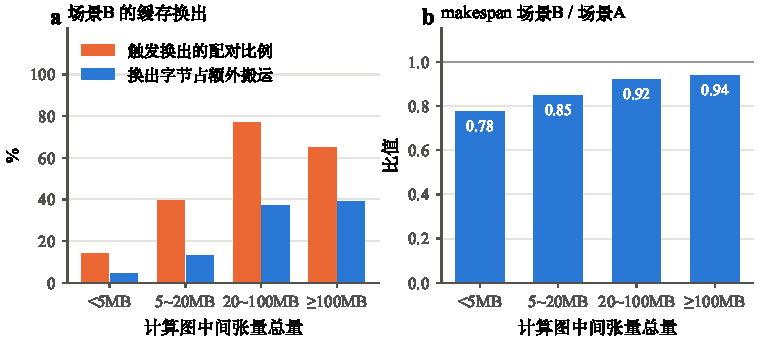
\includegraphics[width=\textwidth]{spill_B}
  \caption{场景 B 的缓存换出。(a) 按中间张量总量分组，触发换出的配对比例与换出字节占额外搬运的比例；(b) 场景 B 相对场景 A 的 Makespan 之比}
  \label{fig:spill}
\end{figure}

综合以上修正，问题二的模型为
\begin{equation}
\begin{aligned}
  \min\quad & M_k=\max_{v\in\Oe} f_v\\
  \text{s.t.}\quad & \text{划分、无环与同核顺序约束 \eqref{eq:assign}--\eqref{eq:order}},\\
  & S_v\ge f_u\ \ (\core(u)=\core(v)),\quad \text{跨核同步约束 \eqref{eq:sync-B}，带宽共享 \eqref{eq:fair-share}},\\
  & f_v\ge S_v+c_v,\quad \text{缓存驻留约束 \eqref{eq:resident}},
\end{aligned}
  \label{eq:obj-p2}
\end{equation}
次要目标为 $Q_B+Q^{\mathrm{sp}}$。它与问题一共用合法性约束，命题~\ref{prop:acyclic} 的结论不变，三种构造算法可以直接使用；变化的是参数的合适区域和后处理的作用。

\subsection{问题二模型求解与结果分析}

\subsubsection{算法描述}

构造阶段沿用算法~\ref{alg:lpt}--\ref{alg:select} 与相同的参数网格，式 \eqref{eq:path-B} 预测最优方案会切得更细：层带数 $W$ 应偏大，相位构造的惩罚 $\lambda$ 此时对应 500 周期同步加上张量传输时间，应比问题一小。\label{sec:p2-coarsen}后处理中，成组合并在场景 B 下的作用需要重新分析。场景 B 下每核本来就只有一个 Task，成组合并既不改变 Task 数，也不改变跨核边界，它改变的是核内执行顺序。评估程序先对整个核的计算图做确定性拓扑排序（题目附录 C 的步骤 1），再按 \texttt{core\_schedules} 中的子图次序做稳定排序：不同子图按给定次序先后排开，同一子图内部保留拓扑排序的相对顺序。把相邻 $w$ 个子图合并后，它们的操作落进同一个桶，按全局拓扑序交错排列，原本前后串行的几条独立链可以穿插执行，张量的驻留区间随之改变，换出量和流水线空闲都可能下降。

除成组合并外，问题二还增加了交叉复评。问题二、三同属场景 B，方案可以互换。我们把问题三各来源的获胜方案交给问题二的评估程序，反之亦然，按方案内容的哈希去重，避免重复评估。它相当于在算法~\ref{alg:select} 的核数补齐之前把候选集扩大为 $\{x\}\cup\{x^{(3)}_{k}\}$，$x^{(3)}_{k}$ 为问题三的已选方案。核数补齐的做法与问题一相同。

\subsubsection{求解分析}

扫描数据支持“场景 B 应切得更细”的判断。图~\ref{fig:nsg} 中问题二的曲线随子图数单调下降：1--3 个子图的候选 Makespan 中位数是该用例最优值的 \V{figx_nsg_p2_median_0} 倍，256 个以上子图的候选只有 \V{figx_nsg_p2_median_4} 倍，5 核最终方案的子图数中位数为 \V{p2_k5_nsg_median}，相位构造胜出的 $\lambda$ 中位数为 \V{p2_phase_bestlam_median}。换核深度仍然起作用，这与式 \eqref{eq:path-B} 一致：图~\ref{fig:depth}(b) 中最终方案的超出量与 $h\,\delta_B$ 的对数相关系数为 \V{figx_depth_p2_corr}，\V{figx_depth_p2_n} 个点中有 \V{figx_depth_p2_above} 个位于对角线上方。也就是说，问题二要控制的是换核深度，而不是子图个数。

表~\ref{tab:algo-p2} 与图~\ref{fig:algocmp}(b) 给出各构造算法与逐用例选优的对比。任何单一算法都落后于选优：5 核时最好的单一算法（分量装箱）为 \V{p2_k5_lpt_mean}，逐用例选优为 \V{p2_k5_portfolio_mean}。层带划分在 I 类上 4 核平均达到 \V{p2_k4_famI_band_mean}，同核层带之间的数据不再往返 DDR，是它在场景 B 中表现好的原因。后处理方面，成组合并在 \V{co1_p2_groups} 组里改进了 \V{co1_p2_improved} 组，平均缩短 \V{co1_p2_mean_red_pct}，最多 \V{co1_p2_max_red_pct}；局部搜索起点可追溯的 \V{ls_p2_jobs} 个作业平均缩短 \V{ls_p2_mean_red_pct}；最终方案中有 \V{source_mix_by_problem_2_crosseval} 组来自交叉复评；核数补齐评估了 \V{mono_p2} 个补空核方案，补齐后每个用例的加速比都随核数单调不减。

\begin{table}[H]
\centering
\caption{问题二：单一构造算法与逐用例选优的平均加速比}
\label{tab:algo-p2}
\renewcommand\arraystretch{1.15}
\begin{tabular}{lcccc}
\toprule
方法 & 2 核 & 3 核 & 4 核 & 5 核 \\
\midrule
朴素基线（分量装箱，$\alpha=0.25$） & \V{p2_k2_naive_mean} & \V{p2_k3_naive_mean} & \V{p2_k4_naive_mean} & \V{p2_k5_naive_mean} \\
分量装箱 & \V{p2_k2_lpt_mean} & \V{p2_k3_lpt_mean} & \V{p2_k4_lpt_mean} & \V{p2_k5_lpt_mean} \\
层带划分 & \V{p2_k2_band_mean} & \V{p2_k3_band_mean} & \V{p2_k4_band_mean} & \V{p2_k5_band_mean} \\
相位构造 & \V{p2_k2_phase_mean} & \V{p2_k3_phase_mean} & \V{p2_k4_phase_mean} & \V{p2_k5_phase_mean} \\
逐用例选优 & \V{p2_k2_portfolio_mean} & \V{p2_k3_portfolio_mean} & \V{p2_k4_portfolio_mean} & \V{p2_k5_portfolio_mean} \\
加后处理（最终） & \V{p2_k2_final_mean} & \V{p2_k3_final_mean} & \V{p2_k4_final_mean} & \V{p2_k5_final_mean} \\
\bottomrule
\end{tabular}
\end{table}

问题二 2--5 核平均加速比依次为 \V{p2_k2_final_mean}、\V{p2_k3_final_mean}、\V{p2_k4_final_mean}、\V{p2_k5_final_mean}（图~\ref{fig:speedup}(b)），5 核相对朴素基线提高 \V{p2_k5_naive_gain_pct}，对可达参考的平均达成率 \V{p2_k5_achieve_mean}。更完整的统计见表~\ref{tab:p2-result}，逐用例结果见附录 B。快速模式下只用 9 个构造候选，2--5 核平均加速比为 \V{figx_fast_p2_k2_mean}、\V{figx_fast_p2_k3_mean}、\V{figx_fast_p2_k4_mean}、\V{figx_fast_p2_k5_mean}，5 核已接近最终结果，在最大用例上一次运行的 CPU 时间约 \V{figx_fast_big_cpu_min} 分钟，满足题目对高效的要求。

\begin{table}[H]
\centering
\caption{问题二结果统计（100 个用例）}
\label{tab:p2-result}
\renewcommand\arraystretch{1.15}
\begin{tabular}{lcccc}
\toprule
 & 2 核 & 3 核 & 4 核 & 5 核 \\
\midrule
平均加速比 & \V{p2_k2_final_mean} & \V{p2_k3_final_mean} & \V{p2_k4_final_mean} & \V{p2_k5_final_mean} \\
最小 / 最大加速比 & \V{p2_k2_final_min} / \V{p2_k2_final_max} & \V{p2_k3_final_min} / \V{p2_k3_final_max} & \V{p2_k4_final_min} / \V{p2_k4_final_max} & \V{p2_k5_final_min} / \V{p2_k5_final_max} \\
平均并行效率 & \V{p2_k2_eff_mean} & \V{p2_k3_eff_mean} & \V{p2_k4_eff_mean} & \V{p2_k5_eff_mean} \\
对可达参考的达成率 & \V{p2_k2_achieve_mean} & \V{p2_k3_achieve_mean} & \V{p2_k4_achieve_mean} & \V{p2_k5_achieve_mean} \\
平均额外搬运量 / MB & \V{p2_k2_added_MB_mean} & \V{p2_k3_added_MB_mean} & \V{p2_k4_added_MB_mean} & \V{p2_k5_added_MB_mean} \\
子图数中位数 & \V{p2_k2_nsg_median} & \V{p2_k3_nsg_median} & \V{p2_k4_nsg_median} & \V{p2_k5_nsg_median} \\
\bottomrule
\end{tabular}
\end{table}

分类别的结果见表~\ref{tab:family}。I 类依赖密集，朴素基线在这一类上几乎等于单核，因为分量装箱以连通分量为单位分核，整张图只有一个分量时所有工作都落在同一个核上；场景 B 下同核子图之间不付代价，只要控制住跨核边，层带划分和相位构造都能在分量内部找到并行性，I 类的提升因此最大。III 类本来就可以按分量并行，朴素基线已经不差，提升空间较小。

\begin{table}[H]
\centering
\caption{问题二各类别的规模与 4 核平均加速比}
\label{tab:family}
\renewcommand\arraystretch{1.15}
\begin{tabular}{lccccc}
\toprule
类别 & 用例数 & 操作数中位 & 宽度比中位 & 朴素基线 & 本文 \\
\midrule
I 单一巨块 & \V{family_count_I} & \V{famI_ops_median} & \V{famI_width_median} & \V{p2_k4_famI_naive_mean} & \V{p2_k4_famI_mean} \\
II 主块+碎片 & \V{family_count_II} & \V{famII_ops_median} & \V{famII_width_median} & \V{p2_k4_famII_naive_mean} & \V{p2_k4_famII_mean} \\
III 多分量 & \V{family_count_III} & \V{famIII_ops_median} & \V{famIII_width_median} & \V{p2_k4_famIII_naive_mean} & \V{p2_k4_famIII_mean} \\
\bottomrule
\end{tabular}
\end{table}

仍以 case\_002 为例。表~\ref{tab:case002} 列出它在问题二下 4 核各构造算法的最优结果。朴素分量装箱的加速比为 1，原因与问题一相同；层带划分只用 $W=\V{cs_p2_band_div}$ 个层带就达到 \V{cs_p2_band_sp}，同核层带之间的数据留在核内，切带不再付出边界往返的代价。这个用例的最优 $W$ 很小，与平均趋势相反，说明参数只能逐用例选。最好的构造仍是相位构造，惩罚取 $\lambda=\V{cs_p2_phase_div}$；最终方案有 \V{cs_p2_final_nsg} 个子图，额外搬运量不到 1~MB。它的逐核时间线见图~\ref{fig:final-tl-p2}：四个核心几乎同时结束，尾部的等待很短，搬运流水线上只剩跨核依赖和图输入输出的搬运，Makespan 为 \V{figx_tl_case_002_p2_ms}。

\begin{table}[H]
\centering
\caption{case\_002 在问题二下的结果（4 核；括号内为胜出参数）}
\label{tab:case002}
\renewcommand\arraystretch{1.15}
\begin{tabular}{lcc}
\toprule
方法 & Makespan & 加速比 \\
\midrule
朴素分量装箱（$\alpha=0.25$） & \V{cs_p2_naive_ms} & \V{cs_p2_naive_sp} \\
分量装箱最优（$\alpha=\V{cs_p2_lpt_div}$） & \V{cs_p2_lpt_ms} & \V{cs_p2_lpt_sp} \\
层带划分最优（$W=\V{cs_p2_band_div}$） & \V{cs_p2_band_ms} & \V{cs_p2_band_sp} \\
相位构造最优（$\lambda=\V{cs_p2_phase_div}$） & \V{cs_p2_phase_ms} & \V{cs_p2_phase_sp} \\
最终方案 & \V{cs_p2_final_ms} & \V{cs_p2_final_sp} \\
\bottomrule
\end{tabular}
\end{table}

\begin{figure}[H]
  \centering
  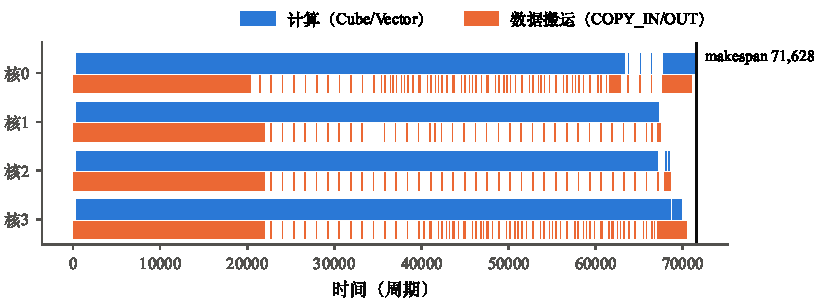
\includegraphics[width=\textwidth]{final_timeline_p2}
  \caption{case\_002 问题二最终方案（4 核）的逐核时间线。每核上条为计算流水线，下条为搬运流水线}
  \label{fig:final-tl-p2}
\end{figure}
